\documentclass{article}

\usepackage[utf8]{inputenc}

\usepackage{nicefrac}
\usepackage{amssymb, amsmath, amsfonts}
\usepackage{amsthm}
\usepackage{tikz}
\usetikzlibrary{matrix,shapes,arrows, calc, intersections}
\usetikzlibrary{decorations.markings}
\usepackage{pgfplots}
\usepackage{tkz-euclide}
\usetkzobj{all} % important you want to use angles
\usepgfplotslibrary{groupplots}
\usepackage[a4paper, margin=1in]{geometry}

\newtheorem{proposition}{Proposition}
\newtheorem{theorem}{Theorem}
\newtheorem{definition}{Definition}
\newtheorem{lemma}{Lemma}
\newtheorem{conjecture}{Conjecture}
\newtheorem{corollary}{Corollary}
\newtheorem{remark}{Remark}
\newtheorem{assumption}{Assumption}

\newlength\figureheight
\newlength\figurewidth
\setlength\figureheight{12cm}
\setlength\figurewidth{14cm}

\newcommand{\tikzdir}[1]{tikz/#1.tikz}
\newcommand{\inputtikz}[1]{\input{\tikzdir{#1}}}

\DeclareMathOperator*{\argmin}{arg\; min}     % argmin
\DeclareMathOperator*{\argmax}{arg\; max}     % argmax
\DeclareMathOperator*{\tr}{tr}     % trace
\DeclareMathOperator{\Cov}{Cov}
\DeclareMathOperator{\logdet}{log\;det}

\title{EE8087 Living with Mathematics\\Tutorial 6: Review}
\date{}
\begin{document} \maketitle
\begin{enumerate}
\item Suppose that $f(x) = \cos(x)+a\cos(x+120^\circ)+b\cos(x+240^\circ)$. If for any $x$, $f(x) = 0$. Determine $a$ and $b$.
\item The triangle $ABC$ is inscribing the rectangle $OPQR$ with points $O,P$ on $AB$ and $Q$ on $BC$ and $R$ on $AC$. If the edge of the triangle has length $a = 5,\,b = 6,\, c = 7$. Find the maximum area of the rectangle $OPQR$.
  \begin{figure}[ht]
    \centering
    \begin{tikzpicture}[scale=0.75]

      \tkzInit[xmax=8, xmin=-1, ymin=-1, ymax=5]
      \tkzClip

      \tkzDefPoint(0,0){A}
      \tkzDefPoint(7,0){B}
      \tkzInterCC[R](A,6cm)(B,5cm)
      \tkzGetPoints{C}{D}
      \tkzDrawPolygon(A,B,C)
      \tkzLabelSegment[below](A,B){$c$}
      \tkzLabelSegment[above](A,C){$b$}
      \tkzLabelSegment[above=1pt](B,C){$a$}

      \tkzDefPoint(2,0){O}
      \tkzDefPoint(2,-1){o}
      \tkzInterLL(O,o)(A,C)\tkzGetPoint{R}
      \tkzDefLine[parallel=through R](A,B) \tkzGetPoint{r}

      \tkzInterLL(R,r)(B,C)\tkzGetPoint{Q}

      \tkzDefLine[parallel=through Q](R,O) \tkzGetPoint{P}
      \tkzDrawPoints(A,B,C,O,R,Q,P)
      \tkzDrawPolygon(O,P,Q,R)
      \tkzLabelPoints(A,B,C,O,R,Q,P)

    \end{tikzpicture}
  \end{figure}

\item The points $A$, $B$, $C$, and $D$ are illustrated in figure below. An engineer wants to use a curve to connect the segment $AB$ and $CD$ and make the connection as smooth as possible. Design a quadratic Bezier curve to achieve this task and find the quadratic equation describing the curve.

  \begin{figure}[ht]
    \centering
    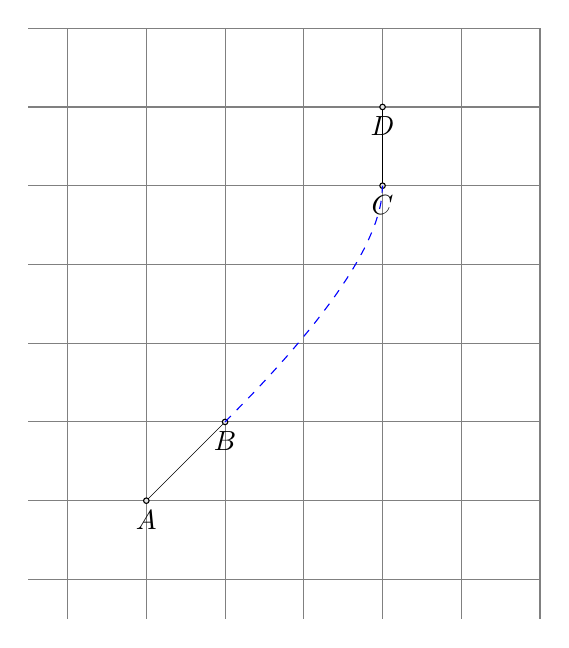
\begin{tikzpicture}
      \tkzInit[xmax=6, xmin=-0.5, ymin=-0.5, ymax=7]
      \tkzAxeXY
      \tkzGrid
      \tkzClip
      \tkzDefPoint(1,1){A}
      \tkzDefPoint(2,2){B}

      \tkzDefPoint(4,5){C}
      \tkzDefPoint(4,6){D}
      \tkzDrawSegments(A,B C,D)
      \tkzDrawPoints(A,B,C,D)
      \tkzLabelPoints(A,B,C,D)
      \draw[domain=0:1, samples=10,smooth,variable=\t,dashed,blue,] plot ({-2*\t*\t+4*\t+2},{-\t*\t+4*\t+2});
    \end{tikzpicture}
  \end{figure}

\item Find the standard form of the quadratic equation $3x^2 - 2xy + 3y^2 + 20x -12y +32 = 0.$
\newpage
\item A driver is driving along a straight highway and she is observing a mountain at point $E$ far away. She first drives $1$km from $A$ to $B$ and observe the apparent shift of $E$ is $\angle AEB = 10^\circ$. She then drives another $2$km and observe the apparent shift of $E$ is $\angle BEC = 20^\circ$. Calculate the distance from $E$ to the highway.

  \begin{figure}[ht]
    \centering
    \begin{tikzpicture}[scale=0.8]
      \tkzInit[xmax=7, xmin=-1, ymin=-1, ymax=12]
      \tkzClip
      \tkzDefPoint(0,0){A}
      \tkzDefPoint(2,0){B}
      \tkzDefPoint(6,0){C}

      \coordinate (p) at (0,{2*tan(80)});
      \coordinate (q) at (2,{4*tan(70)});

      \tkzDefCircle[circum](A,B,p)
      \tkzGetPoint{pp}

      \tkzDefCircle[circum](B,C,q)
      \tkzGetPoint{qq}

      \tkzInterCC(pp,A)(qq,B)
      \tkzGetPoints{E}{F}
      \tkzDrawPoints(A,B,C,E)
      \tkzLabelPoints(A,B,C,E)

      \tkzDrawPolygon(A,C,E)

      \tkzDrawSegment(B,E)

    \end{tikzpicture}
  \end{figure}


\item The orbit of a comet is a conic curve with eccentricity $1.25$. When the comet is at the perihelion point, its distance to the sun is $d$ and its speed is $v$. Calculate the speed of the comet when it is $2.25d$ away from the sun.
\end{enumerate}

\end{document}
%%% Local Variables:
%%% TeX-command-default: "Latexmk"
%%% End:

